\chapter{Analysis of AlphaFold-disorder}
\label{chp:alphafold-disorder}

\section{Introduction}
AlphaFold-disorder is a software tool developed by my co-supervisor Damiano Piovesan, my co-supervisor Alexander Miguel Monzon and other members of the BioComputing UP laboratory. The objective of the software tool is predicting disorder and binding of the aminoacids with high accuracy. 

The web application CAID (Critical Assessment of Protein Intrinsic Disorder), also developed by members of the BioComputing UP laboratory,  was used to measure the quality of the software tool prediction.

In particular 3 algorithms within the tool were measured: 
\begin{itemize}
    \item \textbf{AlphaFold-pLDDT}: uses pLDDT to predict disorder values;
    \item \textbf{AlphaFold-rsa}: uses pLDDT and RSA statistics to predict disorder values;
    \item \textbf{AlphaFold-binding}: uses pLDDT and RSA statistics to predict binding values.
\end{itemize}

Each of these algorithms produces a table containing binding, disorder and other statistics for every aminoacid, or residue\footnote{In molecular biology, a residue refers to a monomer within a polymeric chain. In the case of a protein, a residue refers to an aminoacid.}. 

The professors and researchers of the laboratory published a scientific paper\cite{alphafold-disorder} regarding this software tool: Intrinsic protein disorder and conditional folding in AlphaFoldDB. 

In this chapter we will see more into detail the CAID web application and the 3 algorithms within AlphaFold-disorder.

\section{CAID}
CAID, Critically Assessment of Protein Intrinsic Disorder prediction, is a web application established in 2018 to determine the state-of-art for predicting disorder and binding on IDRs, Intrinsic Disordered Regions. 

The idea is to compare different softwares for this kind of prediction: each of them assigns to every residue of the protein the propensity for that residue to be intrinsically disordered. Accuracy of predictions are evaluated by means of ground truths, obtained by a reference, in this case the reference is the DisProt database. On CAID both software runtimes and accuracy of predictions are compared.

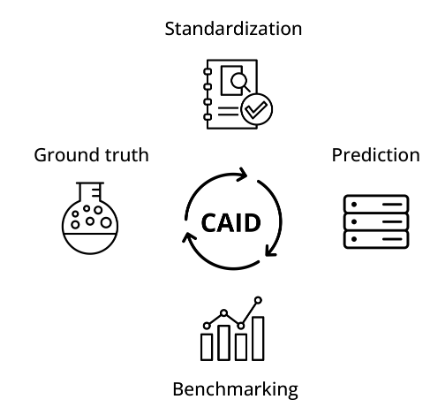
\includegraphics[scale=.5]{res/caid_cycle.png}

Here we can see a picture representing the CAID cycle: Ground Truth, Standardization, Prediction and Benchmarking. Let's analyse them a bit more in detail :
\begin{itemize}
    \item \textbf{Ground Truth}: DisProt database was selected as reference because it contains a large number of manually curated disorder and binding annotations at a protein level. DisProt annotates association between intrinsically disordered regions and a biological function.
    \item \textbf{Standardization}: Participants submit their softwares, and the CAID organizers encapsulate code into containers, providing standardization across different machines. This also makes it easier to deploy them and to package softwares with dependencies.
    \item \textbf{Prediction}: Running the containers implemented in the Standardization step on the Ground Truth targets generates predictions. The cluster used by CAID can execute all methods in parallel within some resource contraints (90 GB RAM, 48 threads, 4 Hours per sequence).
    \item \textbf{Benchmarking}: The performances of the various methods are evaluated by a number of metrics. CAID identifies the confidence threshold to optimize the performance for a specific metric. In benchmarking and runtimes pages are reported some of the assessment results.
\end{itemize}

The 3 algorithms we mentioned earlier: AlphaFold-pLDDT, AlphaFold-rsa and AlphaFold-binding are already present in their containers on the CAID application.

\section{AlphaFold-pLDDT}
This predictor is provided by the software tool AlphaFold-disorder. It's a predictor for disorder, which means that it predicts for each residue its propensity to be intrinsically disordered.

Its predictions are based on the pLDDT, predicted Local Distance Difference Test, which is already present in .pdb files from AlphaFold predictions as the b-factor. So this algorithm just obtains a statistic representing disorder propensity for that residue, out of the b-factor.

AlphaFold-pLDDT uses "1 - pLDDT" as disorder propensity. 

The optimal classification threshold found with CAID is 0.312, representing pLDDT <68.8 \%, this threshold was selected by maximizing the F1-Score performance on the CAID DisProt dataset.
\section{AlphaFold-rsa}
This predictor is provided by the software tool AlphaFold-disorder. This tool, as the last one we talked about, is also a predictor for disorder.

On this predictor, the disorder propensity is calculated with the relative solvent accessibility, RSA, over a local window centered on the residue whose disorder propensity we want to predict. DSSP was used to obtain the relative solvent accessibility and the optimal local window, of 25 residues, was chosen with a grid search in the range of 1 to 50 residues.

The optimal classification threshold for AlphaFold-rsa is of 0.581, which means rsa < 41.9 \%. Again the threshold was selected by maximizing F1-Score performance on the CAID DisProt dataset.

\section{AlphaFold-binding}
Finally we have the last predictor in the software tool AlphaFold-disorder. This is a binding predictor, which means that it predicts a statistic that represents the propensity of a residue to bind.

This predictor makes use of both the pLDDT and the RSA calculated for the other 2 predictors: in the scientific paper \cite{alphafold-disorder} that describes the software tool AlphaFold-disorder, we can see the relation between RSA, pLDDT and this binding propensity.

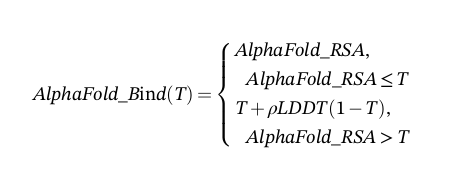
\includegraphics[scale=.7]{res/alphafold-binding.png}

That T represents a threshold, obtained again from maximizing the F1-Score on the CAID DisProt dataset. The optimal threshold found with CAID is 0.773. 

Below 0.773 the binding propensity is the value from AlphaFold-rsa(T); above 0.773 we use the pLDDT score to compute the binding propensity.

\section{Code}
Let's quickly see the most important points in the code of this software tool. The main points are: 
\begin{enumerate}

    \item Parsing of input parameters;
    \item Parsing of input file(s);
    \item Extraction of pLDDT and RSA for each residue;
    \item Computation of predictions;
    \item Creating the output files.
\end{enumerate}
\subsection{Parsing input parameters}
To parse input they used the library parse\_args along with Path and PurePath of the library pathlib.

\begin{lstlisting}[language=Python, caption=import\ libraries\ parsing]
    import argparse
    from pathlib import Path, PurePath
\end{lstlisting}

Parse args it's used to parse parameters given in terminal, when using the software tool. These are the main parameters:
\begin{itemize}
    \item \textbf{-\vspace{0.1cm}-in-struct (-i)}: the input file(s). Either a single file, folder or file listing containing the relative paths of .PDB or .mmCIF files;
    \item \textbf{-\vspace{0.1cm}-out (-o)}: name for the output file(s).
    \item \textbf{-\vspace{0.1cm}-format (-f)}: format for the output file, it can be either "tsv" or "caid";
    \item \textbf{-dssp}: the path for the mkdssp executable, by default is just the alias "mkdssp" which is needed to be setted in the environment variables;
    \item \textbf{-ll}: log level, it can be one of the following: "notset", "debug", "info", "warning", "error", "critical".
\end{itemize}

\begin{lstlisting}[language=Python, caption=Command-line\ arguments\ parsing.]
def parse_args():
    parent_parser = argparse.ArgumentParser(add_help=False)

    group = parent_parser.add_mutually_exclusive_group(required=True)
    group.add_argument('-i', '--in_struct', type=str,
            help='A single file, folder or file listing 
            containing (gzipped) PDB or mmCIF files (relative paths)'
            )   
[...]
    parent_parser.add_argument('-ll', type=str, choices=['notset',
        'debug','info','warning','error','critical'], 
        default='info', help='Log level')
    main_parser = argparse.ArgumentParser(parents=[parent_parser])
    return main_parser.parse_args()
\end{lstlisting}

\subsection{Parsing input files}
First of all the library pathlib is employed to obtain the path of the input file(s) and then we have 4 possibilities, identified through if-else 's :
\begin{itemize}
    \item \textbf{one protein file}: so either a ".pdb" file, a ".pdb.gz", ".cif" or ".cif.gz" file;
    \item \textbf{list of files};
    \item \textbf{a directory}: each protein file within this directory is processed;
    \item \textbf{non-protein files} are recognized and not processed.
\end{itemize}

\begin{lstlisting}[language=Python, caption=Input\ files\ parsing]
if __name__ == '__main__':
    
[...]
    
    p = Path(args.in_struct)
    # args.in_struct is the CLI parameter for input files
    if p.is_file():
        # input is a single struct file or file with list
        if ''.join(PurePath(p).suffixes) in ['.pdb', '.pdb.gz', 
        '.cif', '.cif.gz'] :
            #process single file as input
            processed_data = process_file(p)
[...]
        else:
            # process list of files as input 
            with open(p, 'r') as list_file:
                for file in list_file:
                    real_file = Path(p.parent, Path(file.strip()))
                    processed_data = process_file(real_file)
[...]
    else:
        # input is a directory
        start_T = time.time()
        for file in p.iterdir():
            if ''.join(PurePath(p).suffixes) in ['.pdb', '.pdb.gz',
            '.cif', '.cif.gz'] :
                #process every file in the directory
                processed_data = process_file(p)
\end{lstlisting}


\subsection{Extraction of residues' statistics}

This part is implemented under the main procedure "process\_pdb". To implement this procedure a few libraries have been used: the main ones are BioPython and pandas. The input parameters for the procedure are three:
\begin{itemize}
    \item \textbf{pdb\_file}: the actual protein file, so the path to that file;
    \item \textbf{pdb\_name}: the name of the file;
    \item \textbf{dssp\_path}: the path to the mkdssp executable.
\end{itemize}
\subsubsection{Description of the procedure}
The procedure can be divided in 4 steps :
\begin{description}
    \item \textbf{1. Load structure}: the protein file is loaded and parsed into a proper data structure: "Bio.PDB.Structure", a class in BioPython that represents a macromolecular structure. This parsing is done through "Bio.PDB.PDBParser" if it's a .pdb file or with "Bio.PDB.FastMMCIFParser" if it's a .mmCIF file.
    
    \item \textbf{2. DSSP invokation}: DSSP is a software tool used to obtain interesting statistics for each residue. The software tool is invoked through a Python wrapper\footnote{A wrapper is a class or procedure that translates a library's existing interface into a compatible interface, it "wraps" the underlying library. It's often used to enable cross-language, in this case the wrapper enables the c++ library "DSSP" to be used in Python.} class: "Bio.PDB.DSSP" provided by BioPython. 
    
    \item \textbf{3. Extraction of statistics}: Finally the statistics of interests are extracted by iterating the residues. The statistics of interests are 3: 
    \begin{enumerate}
        \item \textbf{pLDDT}: obtainable without DSSP, from the b-factor value already present in the .pdb file;
        \item \textbf{rsa}: it represents how much the solvent can access this residue. It's provided by DSSP;
        \item \textbf{SS}: secondary structure of the residue. Also provided by DSSP.
    \end{enumerate}
    
    
    \item \textbf{4. Save statistics in a DataFrame}: Finally the statistics of interest are stored in a DataFrame, a class provided by the library "pandas". Dataframe is the most popular way to manage a table and easily write it in a ".csv" or ".tsv" file. 
\end{description}


\subsubsection{Code snippet of the procedure}
For more information on DSSP there is the original scientific paper \cite{og-dssp} and the updated repository of github: \hyperlink{https://github.com/PDB-REDO/dssp}{DSSP}.
Down below we can see an adjusted code snippet to illustrate how this extraction of statistics for each residue works. It's adjusted for the purpose of showing it in this thesis.

\vspace{2em}

\begin{lstlisting}[language=Python, caption=Extraction\ residues'\ statistics]
import pandas as pd
from Bio.PDB import PDBParser, DSSP
from Bio.PDB.MMCIFParser import FastMMCIFParser
from Bio.SeqUtils import seq1
[...]
def process_pdb(pdb_file, pdb_name, dssp_path='mkdssp'):
[...]
    # Load the structure
    file_ext = Path(rel_file).suffix
    if file_ext in ['.pdb']:
        structure = PDBParser().get_structure('', real_file)
    else:
        # assume mmCIF
        structure = FastMMCIFParser().get_structure(''. real_file)
[...]
    # Calculate DSSP. WARNING Check the path of mkdssp
    dssp_dict = dict(DSSP(structure[0], real_file, dssp=dssp_path))
[...]
    # Parse b-factor (pLDDT) and DSSP statistics of interest
    df = []
    for i, residue in enumerate(structure.get_residues()):
        lddt = residue['CA'].get_bfactor() / 100.0
        rsa = float(dssp_dict.get((residue.get_full_id()[2], 
residue.id))[3])
        ss = dssp_dict.get((residue.get_full_id()[2], residue.id))[2]
        df.append((pdb_name, i + 1, seql(residue.get_resname()), 
lddt, 1 - lddt, rsa, ss))
    df = pd.DataFrame(df, columns=['name', 'pos', 'aa', 'lddt', 
'disorder', 'rsa', 'ss'])
    return df
\end{lstlisting}

\section{Usage of AlphaFold-disorder software tool}
\subsection{Dependencies}
In order to use AlphaFold-disorder, we first need :
\begin{itemize}
    \item the actual Python script \textbf{alphafold\_disorder.py};
    \item at least one protein file, in format \textbf{.pdb}, \textbf{.mmCIF}, \textbf{.pdb.gz} or \textbf{.mmCIF.gz};
    \item the DSSP executable: \textbf{mkdssp};
    \item the following libraries: \textbf{BioPython}, \textbf{Numpy} and \textbf{Pandas}.
\end{itemize}
\subsection{Usage}
To execute the software tool we can write the following command in the CLI:
\\
\begin{lstlisting}[language=Bash]
    python3 AlphaFold-disorder -i pdbs/ -o output
\end{lstlisting}
\vspace{1em}
Instead of "output" we can write the name for output file that we desire, and instead of "pdbs/" we can give as input a protein file, a directory containing protein files or a file with the relative paths of protein files.
\vspace{2em}
\subsection{DSSP installation}
There are two ways to install DSSP: 
\begin{enumerate}
    \item Download the pre-compiled file from the  \href{https://github.com/PDB-REDO/dssp/releases/tag/v4.4.0}{latest release in GitHub};
    \item Build the the source file from the GitHub repository.
\end{enumerate}
To build the source file we have to install and build a few libraries, but it's all well-document in the readme.md file of the \href{https://github.com/PDB-REDO/dssp}{DSSP repository}. 

\subsection{Python libraries installation}
To install the 2 Python libraries required we need \textbf{Python3} and \textbf{pip3}, Package Installer for Python. Then to install the 2 Python libraries we just execute the following commands from the CLI:
\begin{itemize}
    \item \textbf{BioPython}: pip3 install biopython;
    \item \textbf{Numpy}: pip3 install numpy;
    \item \textbf{Pandas}: pip3 install pandas.
\end{itemize}